\subsection{~\emph{DSOA}}
\label{subsec:dsoa}
	
		Utilizada no ~\textit{uOS}, o ~\textit{Device Service Oriented Architecture (DSOA)} surgiu como
		uma proposta para auxiliar na modelagem do ambiente inteligente. Essa arquitetura define o modelo
		de comunicação a ser utilizado e trás algumas características definidas pelo ~\textit{Service
		Oriented Architecture (SOA)}, como por exemplo, o reuso dos recursos de software. 
		
		A DSOA define alguns conceitos iniciais:

		\begin{itemize}
			\item Dispositivo

				Um dispositivo é definido como qualquer equipamento que possa prover uma capacidade 
				computacional, ao qual possa hospedar aplicações ou disponibilizar recursos para o ambiente
				inteligente com o objetivo de outras aplicações utilizarem seus serviços.

				Com a evolução da multimídia, muitos equipamentos que até então não estariam de acordo com essa
				definição, como é o caso das televisões ~\textit{SmartTV}, atualmente disponibilizam conexões de
				comunicações, como por exemplo, o ~\textit{Bluetooth} e a ~\textit{Wifi}, que viabilizam seu
				uso no ambiente inteligente. O mesmo acontece com os ~\textit{tablets, celulares}, etc. 
				
			\item Recurso

				Os recursos são definidos como as funcionalidades providas pelos dispositivos. Possuem a
				característica de estarem expostas por interfaces dentro do ambiente, aos quais podem prover
				diversos serviços.

				Tomando como exemplo a ~\textit{SmartTV} do tópico anterior, esse dispositivo oferece dois
				recursos básicos, o de áudio e o de vídeo. Outro dispositivo no ambiente poderia ter um ou mais
				recursos a serem disponibilizados.

			\item Serviço 
				
				O serviço é definido como uma implementação de uma funcionalidade disponibilizada por um recurso
				no ambiente	inteligente. Os serviços são disponibilizados através de uma interface pública
				conhecida, permitindo assim sua utilização entre os dispositivos presentes no
				ambiente inteligente.
				
		\end{itemize}
		
		Para um melhor entendimento com relação aos conceitos apresentados, será apresentado o seguinte
		exemplo:
		
		No ambiente inteligente há uma televisão ~\textit{SmartTV}, esta oferece os recursos de
		áudio e vídeo. A televisão organiza automaticamente a ~\textit{playlist} de áudio em ordem
		alfabética, efetua uma busca na internet para encontrar os álbuns e letras relacionadas a cada
		faixa na contida na ~\textit{playlist} e por fim executa a faixa selecionada.
		
		De acordo com a ~\textit{DSOA}, podemos classificar o exemplo apresentado da seguinte maneira:
		
		\begin{itemize}
		  \item Dispositivo: 
		  
		  		\begin{enumerate}
		  		  \item Televisão ~\textit{SmartTV}
		  		\end{enumerate}
		  
		  \item Recursos: 
			
			  	\begin{enumerate}
			  	  \item Áudio
			  	  \item Vídeo
			  	\end{enumerate}
		  
		  \item Serviços: 
		   
		  		\begin{enumerate}
		  		  \item	Listagem de músicas 
		  		  \item Organização das músicas em ordem alfabética
		  		  \item Busca pela letra da faixa
		  		  \item Busca pelo álbum da faixa
		  		  \item Execução da faixa selecionada
		  		\end{enumerate}
		  		
		\end{itemize}


	A arquitetura ~\textit{DSOA} pode ser vista na figura ~\ref{fig:arquiteturaDSOA}.
	
	\begin{figure}[h]
		\centering 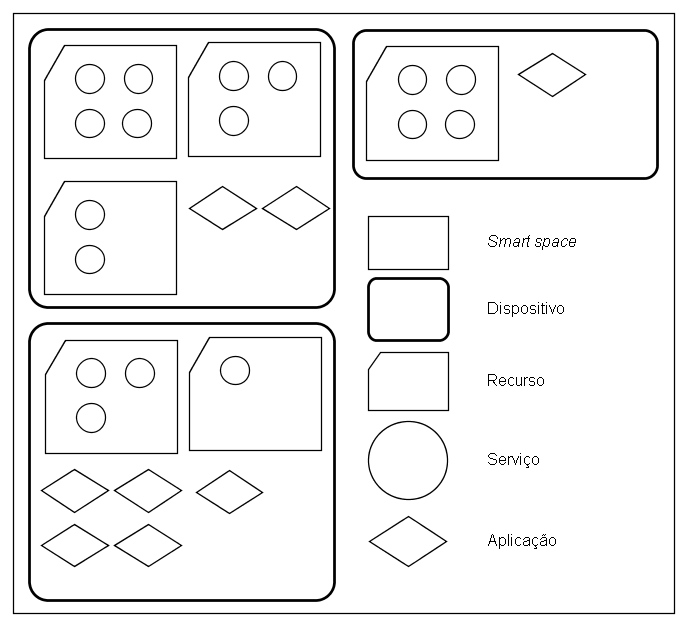
\includegraphics[scale=.5]{figuras/cap3/arquiteturaDSOA.png}
		\caption{\textit{Arquitetura DSOA.}}
		\label{fig:arquiteturaDSOA} 
	\end{figure}

		